% Chapter Template

\chapter{Proposed Methodologies} % Main chapter title

\label{chp:proposed1} % Change X to a consecutive number; for referencing this chapter elsewhere, use~\ref{ChapterX}
In this chapter, a proposed architecture is introduced for detecting COVID-19 that is designed to be lightweight. The architecture is based on two key components: spatial kernel separability and residual connection. By exploiting spatial kernel separability, the number of training parameters is significantly reduced, making the model more computationally efficient. Additionally, residual connections are used extensively to maintain network stability during the training process and to provide the model with regularization effects that reduce overfitting. This combination of spatial kernel separability and residual connections creates a lightweight architecture that is highly effective at detecting COVID-19. Overall, this chapter provides a valuable contribution to the field of COVID-19 detection by introducing a novel and efficient architecture that can help to identify the disease quickly and accurately. 

\begin{figure}[th]
    \centering
    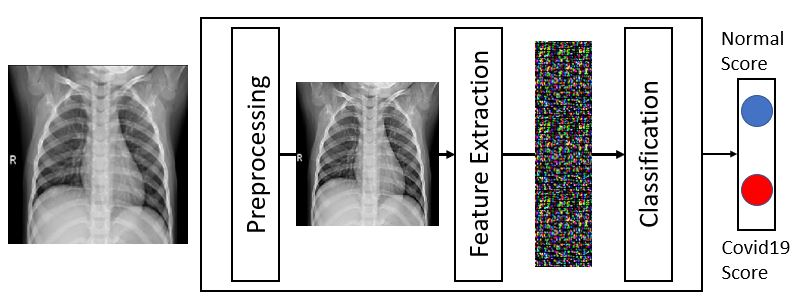
\includegraphics[height=40mm,width=8.0cm]{Figures/fig1.jpg}
    % \decoRule
    \caption{The phases of the proposed method I.}
    \label{fig1}
    \end{figure}

\section{Methodology I}
In this section, a  proposed method I to detect COVID-19 disease from chest X-ray images is presented. The proposed method exploits the CNN model to classify the input chest X-ray image into one of two categories; normal case or Covid-19 case. The proposed method I consists of three phases: preprocessing, feature extraction, and classification. The proposed method phases are shown in Fig.~\ref{fig1}. 

\subsection{Preprocessing Phase}

The preprocessing phase is responsible for resizing and normalizing the input chest X-ray images. The pre-processing phase is employed to maintain the numerical stability of the model and reduce the co-variance shift~\cite{lecun1989handwritten}. In addition, this phase leads the learning model of the CNN model to reduce the required overhead to adapt to the different scales of different features of the input data. Reshaping size is determined empirically. The input chest X-ray image is re-sized and then adapted and normalized to a normal distribution as follows\cite{ioffe2015batch}:

\begin{equation}
Y := \frac{x_i - \mu_{\mathcal B}}{\sqrt{\sigma_{\mathcal B}^2 + \epsilon}}
\label{eq1}
\end{equation}
where $\mu_{\mathcal B}$ and $\sigma_{\mathcal B}^2$ are the mean and standard deviation of chest X-ray image (X), respectively.

After re-sizing the input chest X-ray image, the input image is normalized to have a zero mean and unit standard deviation. Then,  the image can be scaled and shifted with a normalization parameter which is determined and adapted by the training dataset during the training process according to the following equation: 

\begin{equation}
Z := w_1 Y + w_2
\label{eq2}
\end{equation}
where $w_1$ and $w_2$ are a trainable parameter.

Unlike the normalization method presented in~\cite{ioffe2015batch}, the batch normalization process presented in this paper has a $z$-score normalization parameter that is used in both the training and validation phases.


\subsection{Feature Extraction and Classification}

CNN models achieved outstanding success in image recognition~\cite{lecun2015deep}. This phase is responsible for extracting spatial features from the normalized chest X-ray image using a tailored CNN model.  This phase is based on learning the CNN model by the input preprocessed chest X-ray images. The design of the tailored CNN model is described as follows: 

\subsubsection{Separable CNN kernels}
\begin{figure*}
\begin{center}
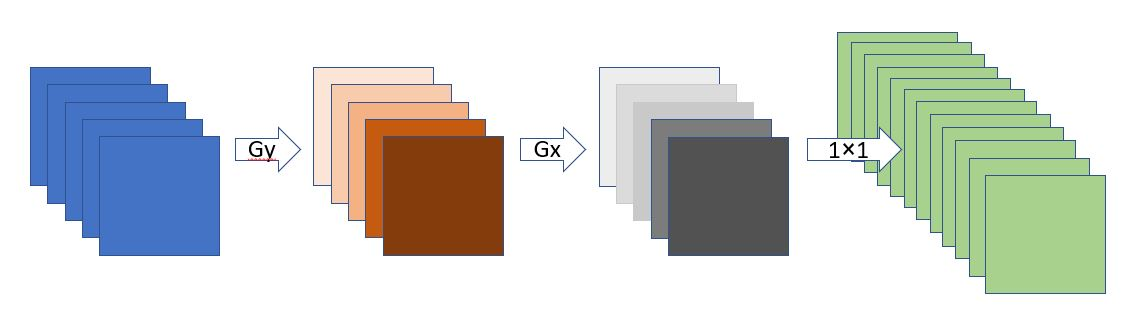
\includegraphics[height=33mm,width=14.0cm]{Figures/fig2.jpg}
\caption{Separable convolution  $Gy$ and $Gx$ have kernel size of $M\times1$ and $1 \times M$.}
\label{fig2}\end{center}\end{figure*}


    
Kernel separability~\cite{rigamonti2013learning}~\cite{szegedy2017inception} is based on decomposing a 2D convolution kernel to linear combinations of two 1D vectors which leads to a large reduction in the total number of resulting parameters. For example, a 2D kernel of size $9 \times 9$ has a total number of $9^2 = 81$  trained parameters. Whereas in the case of separating this 2D kernel to linear combinations of two 1D vectors of sizes $9 \times 1$ and $1 \times 9$, this results in a total number of  $9 + 9 = 18$ trained parameters. As a consequence, kernel separability reduces the number of CNN model operations (such as multiplication and addition). A  2D kernel of $k \times k$ applied for a 2D signal with spatial dimensions of $ M \times N$ has a total number of  $(N-4)(M-4)\times k^2$ operations but in case of applying kernel separability yields $2(N-4)(M-4)k$ operations. The flow of separated convolution operation is summarized in Fig.~\ref{fig2}. The combination of these kernels is approximately a $M\times M$ kernel and depth-wise convolution is applied by a $1\times1$ convolution. The output depth is padded with zeros to have the same spatial size of  $Gy, Gx$. $Gy, Gx$ are performed channel-wise. Fig.~\ref{fig3} represents the structure, denoted by the Separated Convolutional Layer, used in the proposed method with kernel size of $(M\times N)$ and satisfying the convolutional kernel separability. Separated Convolutional Layer is composed of three consecutive layers. The first convolutional layer has a kernel size of $(M\times1)$ and the number of convolutional neurons and filters are equal to the number of channels as the input feature map and the convolution operations are performed channel-wise. The second layer operates in the same way as the first layer but it has a kernel of size $(1\times M)$. The third layer is the convolutional layer with a kernel of size $(1\times1)$ and the number of convolutional neurons is $N$. The collaboration of the three layers are connected to perform similarly to the convolutional layer with a kernel size of $(M\times M)$ and the number of neuron and filter is the same as $N$ but with a large difference in the performance.


\begin{figure}
    \begin{center}
    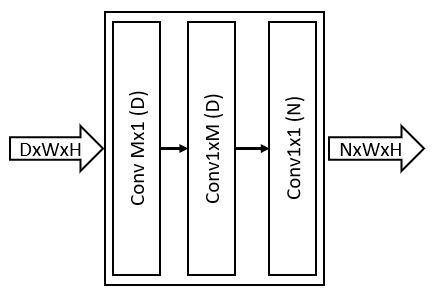
\includegraphics[height=34mm,width=7.0cm]{Figures/fig3.jpg}
    \caption{Separated Convolutional Layer}{ composed of three consecutive layers. The first Convolutional layer has a kernel size of $(M\times1)$ and $D$  convolutional neuron. The second layer operates in the same way as the first layer but it has a kernel of size $(1\times M)$ and $D$ convolutional neuron. The third layer is the convolutional layer with a kernel of size $(1\times1)$ and the number of convolutional neurons is $N$.}
    \label{fig3}
    \end{center}
    \end{figure}

\subsubsection{ Batch Normalization and  Activation function}

In the proposed method linear separable convolutional kernels are followed by a batch normalization and an activation function. Rectified Linear Unit (ReLU)~\cite{he2015delving} is a nonlinear activation that allows the network to fit and approximate highly non-linear dataset distribution. The proposed method employs batch normalization which is described in~\cite{ioffe2015batch}. 

Batch Normalization~\cite{ioffe2015batch} reduces internal covariate shift produced as a result of moving between layers during the feedforward procedure~\cite{ioffe2015batch}. Batch Normalization makes the loss landscape smoother and reduces the number of saddle points~\cite{santurkar2018does} which allows to use of higher learning rates. Using a higher learning rate makes the network training  faster~\cite{ioffe2015batch}. Batch normalization reduces the vanishing gradient problem and exploding gradient problem as it makes the resulted activation scale independent from the trainable parameter scale~\cite{ioffe2015batch}. Batch normalization has the effect of regularization because of the inherited randomness when selecting the batch sample~\cite{ioffe2015batch} which help the generalization to unseen chest X-ray image.

\subsubsection{ Deep and larger receptive field Network design}

Deeper convolutional neural network design is a very important task for any image recognition task~\cite{he2016deep}. Training a deeper network is very expensive and has many challenges such as vanishing gradient problem, exploding gradient problem, and degradation problem~\cite{he2016deep}. The exploding gradient problem occurs when the gradient update becomes very large (approaching infinity) resulting in the network diversion. A vanishing gradient problem occurs when the gradient update becomes very small (approaching zero) resulting in preventing the parameter update for early layers~\cite{ioffe2015batch} and preventing the network from learning new patterns. Batch normalization~\cite{ioffe2015batch} and the use of ReLU activation function~\cite{krizhevsky2012imagenet} alleviate these two problems.

The deep layers of CNN networks sometimes need to approximate the identity function which is not a simple task, especially with the existence of a non-linear function. Residual connection~\cite{he2016deep} overcomes this problem by using skip connection as shown in Fig.~\ref{fig4}.
Fig.~\ref{fig4} represents the building block layer of the feature extraction phase, denoted by a stack of Residual Separated Block  (RSB). RSB consists of four layers of separated convolutional layers, each layer is followed by a batch normalization and an activation function. It has an output of depth $N$ where each sublayer produces an output of depth $N/4$ which is concatenated at the end of the layer to produce a depth  $N$. RSB produces a feature map that includes both low-level features and high-level features.

\begin{figure*}
\begin{center}
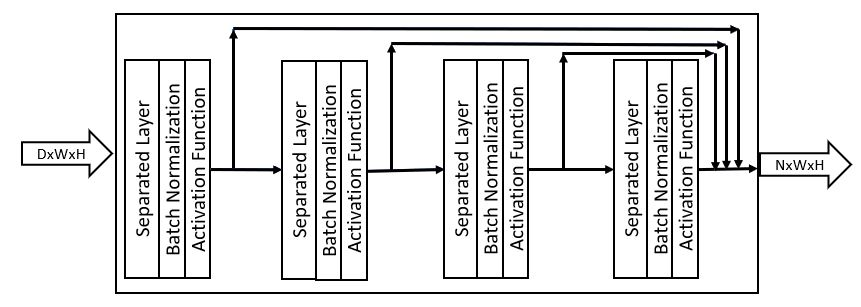
\includegraphics[height=38mm,width=14.0cm]{Figures/fig4.jpg}
\caption{The stack of residual separated block  (RSB) consists of four layers of separated convolutional layer each of which is followed by batch normalization and activation function. Feature maps are concatenated at the end of the block.}
\label{fig4}
\end{center}
\end{figure*}

\begin{figure*}
    \begin{center}
    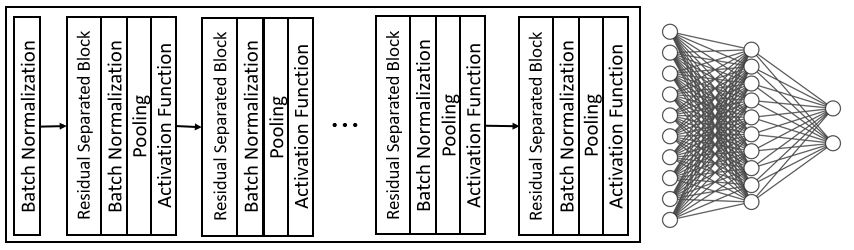
\includegraphics[height=37mm,width=14.0cm]{Figures/fig5.jpg}
    \caption{The complete proposed tailored CNN architecture.}
    \label{fig52}
    \end{center}
    \end{figure*}
    
Unlike the traditional neural network, which is fully connected to the previous layer, the convolutional neural network is connected locally to a local region of the previous feature map. This introduces the concept of the network receptive field~\cite{luo2016understanding}. The receptive field should be large enough to capture large patterns in the input chest X-ray image. Therefore, any consecutive convolutional layers in the proposed method without a pooling layer in between a larger kernel size are used in one of them. Residual Separated block, RSB, in Fig.~\ref{fig4} may have kernel sizes of 3, 5, 7, and 9, respectively.\\
Figure.~\ref{fig52} Represent a complete CNN architecture.

% \section{Summary}
% % In this chapter a lightweight CNN architecture is proposed for COVID-19 detection. The proposed architecture is based on the spatial separability of the convolutional kernel to enforce the learning of linear kernels. The proposed architecture consists of separated kernels of convolutional layers that are connected by a residual connection. The proposed architecture uses batch normalization to maintain network stability during the training process.


% % In this chapter, a novel lightweight CNN architecture is proposed for COVID-19 detection that is based on the concept of spatial kernel separability. The proposed architecture is designed to reduce the number of training parameters and improve computational efficiency by exploiting the separability of convolutional kernels. By learning linear kernels, the model can perform faster and more accurately on the given dataset. The proposed architecture includes separated kernel convolutional layers that are connected by a residual connection, which helps maintain network stability during training. Additionally, the proposed architecture utilizes batch normalization, a technique that helps to standardize the inputs of each layer and improve the convergence rate of the model. By combining these techniques, the proposed architecture offers a lightweight, efficient, and accurate method for detecting COVID-19.
% In this chapter, the proposed lightweight CNN architecture for COVID-19 detection is designed with the concept of spatial separability in mind. The spatial separability of the convolutional kernel is used to enforce the learning of linear kernels, which reduces the number of training parameters and improves computational efficiency. Essentially, the model is designed to recognize patterns in the data that are linearly separable, which enables the use of simpler and more efficient models.

% The proposed architecture comprises separated kernel convolutional layers that are connected by a residual connection. The use of separated kernel convolutional layers helps to reduce the number of training parameters, while the residual connection improves network stability during the training process. The residual connection enables the model to retain important features while also discarding unimportant ones, which helps prevent overfitting.

% Batch normalization is used in the proposed architecture to maintain network stability during the training process. The technique standardizes the inputs of each layer, which improves the convergence rate of the model. This is done by normalizing the layer inputs to have zero mean and unit variance, which helps prevent internal covariate shifts. Internal covariate shift refers to the change in the distribution of network activations that occurs during training, which can slow down the convergence rate.

% In summary, the proposed lightweight CNN architecture for COVID-19 detection is based on the spatial separability of the convolutional kernel, with separated kernel convolutional layers connected by a residual connection. Batch normalization is used to maintain network stability during training, which improves the convergence rate of the model. By combining these techniques, the proposed architecture offers an efficient, accurate, and stable method for detecting COVID-19.